\chapter{Compléments sur le détecteur et l'identification hadronique}
\label{app:detecteur}

Cette annexe regroupe des éléments écartés du corps du mémoire : les caractéristiques de
l'électronique de lecture du prototype, le tableau comparatif des signatures calorimétriques
attendues pour les trois espèces étudiées, et les corrélations entre variables d'entrée des
modèles d'apprentissage.

\section{Électronique de lecture et acquisition}
\label{app:electronique}

L'électronique de lecture est intégrée au plus près des chambres grâce aux ASICs
\textsc{HARDROC} \cite{dulucq2010hardroc}, conçus pour les détecteurs gazeux hautement segmentés.
Chaque ASIC gère plusieurs dizaines de canaux et dispose d'une mémoire locale permettant de stocker
les informations avant la lecture.

Cette architecture embarquée réduit le câblage externe et rend possible l'instrumentation d'un très
grand nombre de canaux. Le système peut fonctionner en mode déclenché ou en mode sans déclenchement,
selon les conditions expérimentales.

Une stratégie de \emph{power pulsing} peut également être utilisée afin de réduire la consommation
électrique pendant les périodes sans faisceau, un point important pour les futurs collisionneurs
linéaires.

\section{Signatures calorimétriques attendues}
\label{app:signatures}

Le Tableau~\ref{tab:comparaison-signatures} détaille, espèce par espèce, les signatures moyennes
attendues dans le SDHCAL à partir des différences physiques discutées à la
section~\ref{sec:pid-enjeux}. Ces tendances sont statistiques : les fortes fluctuations des gerbes
hadroniques font que les distributions correspondantes se recouvrent largement événement par
événement, ce qui est précisément la difficulté que doit surmonter le classificateur.

\begin{table}[!ht]
    \centering
    \caption{Comparaison qualitative des signatures calorimétriques moyennes attendues dans le SDHCAL.}
    \label{tab:comparaison-signatures}
    \renewcommand{\arraystretch}{1.4}
    \resizebox{\textwidth}{!}{%
    \begin{tabular}{lccc}
        \hline
        \textbf{Caractéristique} &
        \textbf{Pion $\pi^-$} &
        \textbf{Proton $p$} &
        \textbf{Kaon neutre long $K^0_L$} \\
        \hline
        Signal d'ionisation avant gerbe    & Oui               & Oui               & Non \\
        Fraction électromagnétique moyenne & Élevée            & Plus faible       & Variable \\
        Profondeur de première interaction & Plutôt précoce    & Plutôt précoce    & Plus variable \\
        Développement longitudinal         & Relativement précoce & Plus profond   & Variable \\
        Extension transverse               & Modérée           & Plus large        & Variable \\
        Fluctuations événement/événement   & Importantes       & Importantes       & Très importantes \\
        \hline
    \end{tabular}%
    }
\end{table}

\section{Corrélations entre variables d'entrée}
\label{app:correlations}

La Figure~\ref{fig:corr-matrix} présente la matrice de corrélation de Pearson calculée sur
l'ensemble des variables d'entrée des modèles d'apprentissage, tous événements confondus. Plusieurs
groupes cohérents s'y dessinent, qui correspondent aux familles de descripteurs définies en
Annexe~\ref{annexe:showeranalyzer}.

Les variables d'\textbf{activité globale et de compacité} — \texttt{Thr1}, \texttt{Thr2},
\texttt{Thr3}, \texttt{NClusters}, \texttt{Nmax}, \texttt{AvgClustSize}, \texttt{MaxClustSize} et
\texttt{Density} — présentent des corrélations modérées à fortes, ce qui est attendu puisqu'elles
mesurent toutes, sous des formes différentes, l'intensité locale ou globale de la gerbe. Les
descripteurs \textbf{longitudinaux} (\texttt{Begin}, \texttt{Zbary}, \texttt{Zrms}, \texttt{Xmax},
\texttt{z0\_fit}) sont positivement corrélés entre eux, décrivant conjointement la position de départ
et l'évolution de la cascade en profondeur. Les variables de \textbf{forme géométrique}
(\(\lambda_1\), \(\lambda_2\), \texttt{eccentricity3D}) sont liées par leur rôle commun dans la
description de l'anisotropie spatiale. Les variables \textbf{temporelles} (\texttt{tMin},
\texttt{tMean}, \texttt{tSpread}), enfin, ne sont que faiblement à modérément corrélées entre elles,
mais montrent certains liens avec les variables longitudinales — ce qui suggère une connexion entre
chronologie du signal et profondeur d'initiation de la gerbe.

Cette organisation indique que plusieurs variables transportent une information partiellement
redondante. Une sélection plus compacte des observables — en conservant un représentant robuste par
groupe corrélé, par exemple \texttt{Thr3} ou \texttt{Nmax}, \texttt{Density} ou \texttt{NClusters} —
pourrait donc être envisagée sans perte majeure de performance, avec le bénéfice d'une dimension
réduite, d'un entraînement plus rapide et d'une interprétation physique plus lisible.

\begin{figure}[!ht]
  \centering
  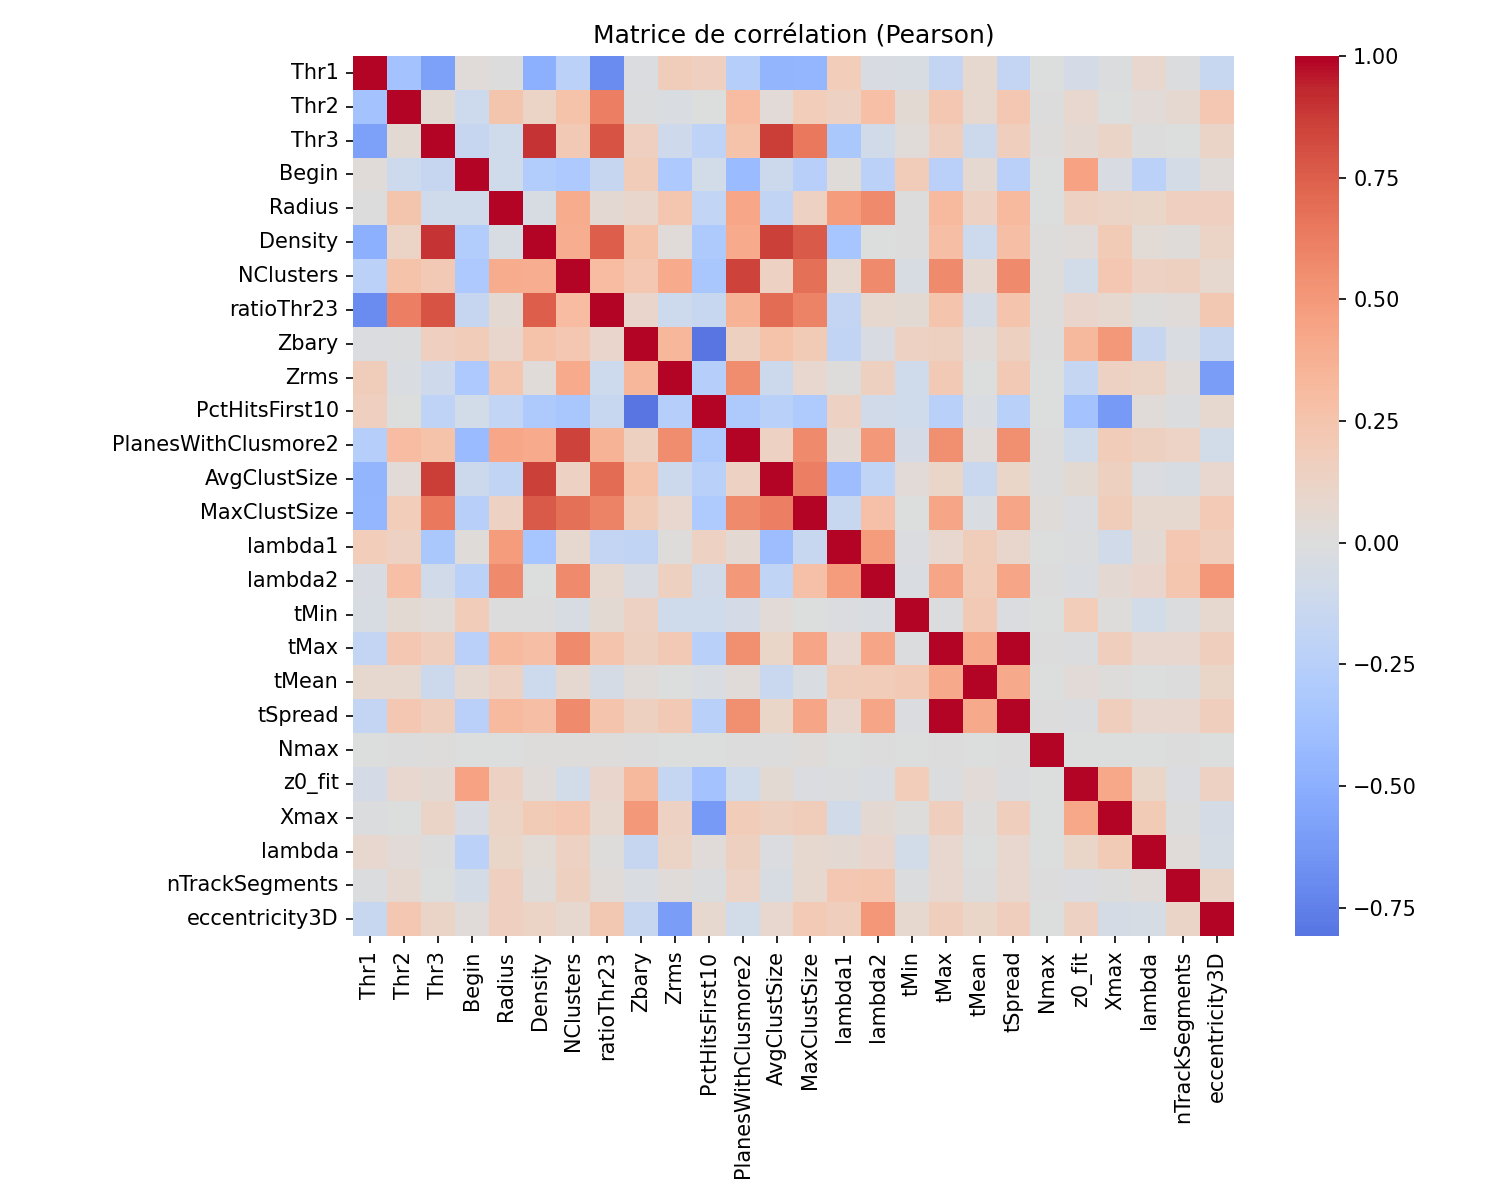
\includegraphics[width=0.72\linewidth]{Fig/correlation_matrix.png}
  \caption{Matrice de corrélation de Pearson des variables d'entrée utilisées pour la
           classification.}
  \label{fig:corr-matrix}
\end{figure}

